%% For double-blind review submission, w/o CCS and ACM Reference (max submission space)
\documentclass[acmsmall,review,anonymous,nonacm]{acmart}\settopmatter{printfolios=true,printccs=false,printacmref=false}
%% For double-blind review submission, w/ CCS and ACM Reference
%\documentclass[acmsmall,review,anonymous]{acmart}\settopmatter{printfolios=true}
%% For single-blind review submission, w/o CCS and ACM Reference (max submission space)
%\documentclass[acmsmall,review]{acmart}\settopmatter{printfolios=true,printccs=false,printacmref=false}
%% For single-blind review submission, w/ CCS and ACM Reference
%\documentclass[acmsmall,review]{acmart}\settopmatter{printfolios=true}
%% For final camera-ready submission, w/ required CCS and ACM Reference
%\documentclass[acmsmall]{acmart}\settopmatter{}


%% Journal information
%% Supplied to authors by publisher for camera-ready submission;
%% use defaults for review submission.
\acmJournal{PACMPL}
\acmVolume{1}
\acmNumber{POPL} % CONF = POPL or ICFP or OOPSLA
\acmArticle{1}
\acmYear{2021}
\acmMonth{1}
\acmDOI{} % \acmDOI{10.1145/nnnnnnn.nnnnnnn}
\startPage{1}

%% Copyright information
%% Supplied to authors (based on authors' rights management selection;
%% see authors.acm.org) by publisher for camera-ready submission;
%% use 'none' for review submission.
\setcopyright{none}
%\setcopyright{acmcopyright}
%\setcopyright{acmlicensed}
%\setcopyright{rightsretained}
%\copyrightyear{2018}           %% If different from \acmYear

\bibliographystyle{ACM-Reference-Format}
\citestyle{acmauthoryear}

\renewcommand{\topfraction}{1} % Allow floats to take up the page
\renewcommand{\textfraction}{0}


%% Packages
\usepackage{booktabs}
\usepackage{subcaption}
\usepackage{graphicx}

% Support \includegraphics of .dot files
\DeclareGraphicsRule{.dot}{pdf}{.pdf}{`dot -Tpdf #1 -o \noexpand\OutputFile}


%%%%%%%%
% TikZ Stuff
%\usepackage{etex} % Fix "No room for new \dimen" error
\usepackage{shellesc} % Fix bug that breaks the tikz 'external' library
\usepackage{tikz}
\usetikzlibrary{babel} % Ensure compatibility the 'babel' package

\usetikzlibrary{external} % Needs to be separately enabled
%\tikzexternalize % Enable externalization
%\usepackage{lua-visual-debug}

\usetikzlibrary{arrows.meta} % Arrow Tips
\tikzset{>=Stealth}
%\tikzset{<=stealth}
%\tikzset{arrows={-Stealth[scale=50]}}
%\tikzset{edge from parent/.style={draw,->,line width=0.6pt}}
%\tikzset{wideline/.style={line width=0.7pt}}
%\tikzset{boldline/.style={color=black,line width=1.0pt}}

\usetikzlibrary{
  graphs,       % Graph *notation*
  graphdrawing, % Graph *layout*
}

\usegdlibrary{
  trees,
}

\begin{document}

%% Title information
\title[Grove]{Grove: A Convergent Collaborative Structure-Editor Calculus}
%\subtitle{Subtitle}

%% Author information
\author{Michael D. Adams}
\orcid{0000-0003-3160-6972}

\author{Eric Griffis}
\orcid{nnnn-nnnn-nnnn-nnnn}

\author{Cyrus Omar}
\orcid{0000-0003-4502-7971}
\affiliation{
  \position{Assistant Research Scientist}
  \department[0]{Computer Science and Engineering}
  \department[1]{Electrical Engineering and Computer Science}
  \department[2]{College of Engineering}
  \institution{University of Michigan}
  \streetaddress{Bob and Betty Beyster Building, 2260 Hayward Street}
  \city{Ann Arbor}
  \state{MI}
  \postcode{48109-2121}
  \country{USA}
}


%% Abstract
%% Note: \begin{abstract}...\end{abstract} environment must come
%% before \maketitle command
\begin{abstract}
Text of abstract \ldots.
\end{abstract}


%% 2012 ACM Computing Classification System (CSS) concepts
%% Generate at 'http://dl.acm.org/ccs/ccs.cfm'.
%\begin{CCSXML}
%<ccs2012>
%<concept>
%<concept_id>10011007.10011006.10011008</concept_id>
%<concept_desc>Software and its engineering~General programming languages</concept_desc>
%<concept_significance>500</concept_significance>
%</concept>
%<concept>
%<concept_id>10003456.10003457.10003521.10003525</concept_id>
%<concept_desc>Social and professional topics~History of programming languages</concept_desc>
%<concept_significance>300</concept_significance>
%</concept>
%</ccs2012>
%\end{CCSXML}
%\ccsdesc[500]{Software and its engineering~General programming languages}
%\ccsdesc[300]{Social and professional topics~History of programming languages}
%% End of generated code


%% Keywords
%% comma separated list
% \keywords{keyword1, keyword2, keyword3}  %% \keywords are mandatory in final camera-ready submission


%% \maketitle
%% Note: \maketitle command must come after title commands, author
%% commands, abstract environment, Computing Classification System
%% environment and commands, and keywords command.
\maketitle


\section{Introduction}
\label{sec:introduction}

Motivation: 
- collaborative editing (both synchronous ala Google Docs and asynchronous version control) 
  is good and important as computing grows
- semantic structure editing is good because it solves the gap problem (semantic editor services 
  are always available) -- cite Hazelnut papers (talk about holes)
- previous approaches to collaborative editing have limitations
  - diff/merge based approaches (trying to solve the inverse problem based on final states -- 
    you lose the actual actions that were performed, and have to reconstruct them or an approx.
    of them i.e. add line/delete line actions -- would need to adapt this to structure editing,
    some papers have started to look at that, but fundamentally we don't want to throw away the
    knowledge we have about the edits!)
  - operational transforms (complexity, you have to patch previous actions based on new actions)
  - CRDT-based collaborative editing (that's all been on text, not PL semantics) -- this is good
    because it is relatively simple: you just send all the edits to all the replicas and they are 
    convergent by design
- we want to have the same convergence for a CRDT-based collaborative structure editor that maintains
  the sensibility invariant of Hazelnut, i.e. every editor state has meaning. mention that maintaining sensibility 
  allows scaling of semantic editor services in the presence of large number of collaborators (in contrast,
  using VS Code or other collaborative text editors with large numbers of collaborators means that almost always
  the semantic editor services will be disabled because the program is going to be broken in multiple places
  transiently)

  this is tricky because:
  - some edits might be conflicting -- solve this with "conflict holes"
  - adding cut/paste or delete/restore allows for degenerate programs (cycles, multiple parents, etc.)
- since we are commutative, we solve both synchronus and async collaborative editing
  - and this resolves issues around merges and conflicts
- contribution of this paper is to solve these problems from type-theoretic first principles:
  - ...
- Hazel

\subsection{Contributions and Paper Organization}
\label{sec:paper-organization}

\section{Grove By Example}
\label{sec:grove-by-example}

TODO: gray-scale unchanged parts of diagrams

TODO: somewhere in here, maybe multiple places, we want to talk about typing the intermediate states that arise

TODO: annotate vertexes and edges with ids (gray superscript?)

Single User Intuition:
 - manipulating trees,
 - holes

Multi User Intuition:
 - vertexes have unique ids
 - edits create or delete edges in the tree,
 - vertexes are automatically created when an edge goes to it
 
Deeper intuition:
 - edges have unique ids
 - once deleted an edge can never be recreated (though, a new edge (with a new id) can be created in the same spot as the original)

\subsection{Scenario X: Holes in the Tree}
\label{sub:Holes in the Tree}

\begin{figure}
\centering 
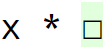
\includegraphics{graphviz/simple.dot}
\begin{tikzpicture}
% TODO: texttt
% TODO: position the different graphs
\path (0cm,0cm) graph[tree layout] {
  + -> {
    2[as={\texttt{2}}],
    % <empty>
  }
};
\end{tikzpicture}
\caption{Scenario X: Holes in the Tree}
\label{fig:Scenario X: Holes in the Tree}
\end{figure}

DIAGRAM: 2 + HOLE

NEEDS UI EXAMPLE

\subsection{Scenario A: Editing Different Parts of the Code}

\begin{figure}
\centering
TODO: commutativity diagram of screenshots with two cursors
\caption{TODO:Caption}
\label{fig:Screenshot0}
\end{figure}

\begin{figure}
\centering
\begin{tikzpicture}
% TODO: texttt
% TODO: position the different graphs
\path (0cm,0cm) graph[tree layout] {
  + -> {
    3[as={\texttt{3}}], % TODO: put a cursor (green) here
    4 % TODO: put a cursor (red) here
  }
};
\path (-3cm,-2cm) graph[tree layout] {
  + -> {
    13, % TODO: put a cursor here
    4
  }
};
\path (3cm,-2cm) graph[tree layout] {
  + -> {
    3,
    14 % TODO: put a cursor here
  }
};
\path (0cm,-4cm) graph[tree layout] {
  + -> {
    13, % TODO: put a cursor here
    14 % TODO: put a cursor here
  }
};
\end{tikzpicture}
\caption{Scenario A: Editing Different Parts of the Code}
\label{fig:Scenario A: Editing Different Parts of the Code}
\end{figure}

A + B make edits and transmit to C, C is able to resolve without any assistance, 
order that the edits are received doesn't matter you get the same program state
at the end

\subsection{Scenario B: Edits to Nested Parts of the Code}

\begin{figure}
\centering
\begin{tikzpicture}
% TODO: texttt
% TODO: position the different graphs
\path (0cm,0cm) graph[tree layout] {
  lam[as={$\lambda_{\texttt{x}}$}] -> {
    * -> {
      2,
      x
    }
  }
};
\path (-3cm,-2cm) graph[tree layout] {
  lam[as={$\lambda_{\texttt{x}}$}] -> {
    + -> {
      1,
      * -> {
        2,
        x
      }
    }
  }
};
\path (3cm,-2cm) graph[tree layout] {
  lam[as={$\lambda_{\texttt{x}}$}] -> {
    * -> {
      3,
      x
    }
  }
};
\path (0cm,-4cm) graph[tree layout] {
  lam[as={$\lambda_{\texttt{x}}$}] -> {
    + -> {
      1,
      * -> {
        3,
        x
      }
    }
  }
};
\end{tikzpicture}
\caption{Scenario B: Edits to Nested Parts of the Code}
\label{fig:Schenario-B}
\end{figure}

TODO: REDO to MOVE a SUBTREE

NEEDS UI MOCKUP

A edits part of the code

B moves the code surrounding the edits of A to another part of the code

Contrast with a traditional diff

\subsection{Scenario C: Direct Conflicts}

\begin{figure}
\centering
\begin{tikzpicture}
% TODO: texttt
% TODO: position the different graphs
\path (0cm,0cm) graph[tree layout] {
  lam[as={$\lambda_{\texttt{x}}$}] -> {
    x
  }
};
\path (-3cm,-2cm) graph[tree layout] {
  lam[as={$\lambda_{\texttt{x}}$}] -> {
    + -> {
      1,
      x
    }
  }
};
\path (3cm,-2cm) graph[tree layout] {
  lam[as={$\lambda_{\texttt{x}}$}] -> {
    * -> {
      x,
      2
    }
  }
};
\path (0cm,-4cm) graph[tree layout] {
  lam[as={$\lambda_{\texttt{x}}$}] -> {
    + -> {
      1,
      x
    },
    * -> {
      x,
      2
    }
  }
};
\path (2cm,-8cm) graph[tree layout] {
  lam[as={$\lambda_{\texttt{x}}$}] -> {
    + -> {
      1,
      * -> {
        x,
        2
      }
    }
  }
};
\path (-2cm,-8cm) graph[tree layout] {
  lam[as={$\lambda_{\texttt{x}}$}] -> {
    * -> {
      + -> {
        1,
        x
      },
      2
    }
  }
};
\end{tikzpicture}
\caption{Scenario C: Direct Conflicts}
\label{fig:Scenario-C}
\end{figure}

DIAGRAM: lam x. x

DIAGRAM: lam x. 1 + x

DIAGRAM: lam x. 2 * x

DIAGRAM: Merge: diamond with "1 +" and "2 *"

TODO: SHOW intermediate Steps (maybe no graph)
  Show user's perspective
  Accept one side = delete others (select this)
  Delete x in *
  Move + to x
  
UI Level Move = Delete and Add

DIAGRAM: Resolution \#1: lam x. 1 + 2 * x

DIAGRAM: Resolution \#2: lam x. 2 * (1 + x)

NEEDS UI MOCKUP

Say: "might not be a popup"

A and B both insert different expressions into the same hole

(think about critiques re: diff)

(compare to what happens when there are conflicts in a VCS, you get 
diff markers inserted into files and the semantic editor services 
no longer understand the code)

\subsection{Scenario D: Deletion of Code Being Edited}

\begin{figure}
\centering
\begin{tikzpicture}
% TODO: texttt
% TODO: position the different graphs
\path (0cm,0cm) graph[tree layout] {
  lam[as={$\lambda_{\texttt{x}}$}] -> {
    + -> {
      2,
      x
    }
  }
};
\path (-3cm,-2cm) graph[tree layout] {
  lam[as={$\lambda_{\texttt{x}}$}] -> {
    + -> {
      3,
      x
    }
  }
};
\path (3cm,-2cm) graph[tree layout] {
  lam[as={$\lambda_{\texttt{x}}$}] -> {
    hole
    },
  + -> {
    2,
    x
  }
};
\path (0cm,-4cm) graph[tree layout] {
  lam[as={$\lambda_{\texttt{x}}$}] -> {
    hole
    },
  + -> {
    3,
    x
  }
};
\end{tikzpicture}
\caption{Scenario D: Deletion of Code Being Edited}
\label{fig:Scenario-D}
\end{figure}

TODO: move into Scenario B

DIAGRAM: lam x. 2 + x

DIAGRAM: (lam x. HOLE) (2 + x)

DIAGRAM: lam x. 3 + x

DIAGRAM: Merge: (lam x. HOLE) (3 + x)

NEEDS UI MOCKUP

A deletes code that B is editing (introduce notion of identity)



(orphans)

Figure shared between D and E that shows the deleted nodes and restore button

\subsection{Scenario E: Restoring Deleted Code}

Combine with Scenario B (moving code):
  delete
  restore
  cut/paste (i.e., move) = delete then restore
  copy structure vs copy id
  paste structure vs paste id
    (show two or three options at paste time)

DIAGRAM: 1 * 2 + 3 + HOLE

DIAGRAM: HOLE + 3 + HOLE (1 * 2)

DIAGRAM: HOLE + 3 + 1 * 2

NEEDS UI MOCKUP

If only one restore, then it does what you expect (basically a cut and paste)

If multiple replicas restore to different places, then you get some complexity:

 -- restore isn't a copy, it is a move

Multi-parent

Cycles

(Maybe not in initial grove by example) The A and B diamond example

\subsection{Scenario F: Cycles}

Synthetic cycles:

DIAGRAM: restoring into yourself (paste before delete?)

Organic cycles:

DIAGRAM: 

NEEDS UI MOCKUP


\section{Formalism}
\label{sec:formalism}

\subsection{Syntax}

\subsection{Convergent Graphs}

Graph CRDT description

Mapping of syntax into the graph representation

Graph actions

holes are not explicit in the graph

\begin{theorem}[Commutativity (convergence?)]

\end{theorem}

\subsection{Type System}
\label{sub:type-system}

conflicts (multiple children in the same spot)

multi-parent

cycles

non-empty holes

\subsection{Semantic Actions}
Mapping to graph actions

Sensibility

\subsection{Agda Mechanization}
\label{sub:agda-mechanization}

\section{Implementation}
\label{sec:implementation}
GRV -- how it is implemented, how it connects to the formalism, describe the graph, 

We implemented GRV as a core OCaml library in approximately 1,500 lines of code, and a basic Web interface in approximately 600 lines of OCaml code and 250 lines of HTML+CSS+Javascript.

Compared to the core language, our implementation lacks support for lists and case expressions.

Optimizations: least fixed point 

\section{Related Work}
\label{sec:related-work}

Hazel

CRDTs

Pidjul

Etherpad

Live Share

Git

Darcs

Unision?

\section{Discussion and Conclusion}
\label{sec:conclusion}


%% Acknowledgments
\begin{acks}                            %% acks environment is optional
                                        %% contents suppressed with 'anonymous'
  %% Commands \grantsponsor{<sponsorID>}{<name>}{<url>} and
  %% \grantnum[<url>]{<sponsorID>}{<number>} should be used to
  %% acknowledge financial support and will be used by metadata
  %% extraction tools.
  This material is based upon work supported by the
  \grantsponsor{GS100000001}{National Science
    Foundation}{http://dx.doi.org/10.13039/100000001} under Grant
  No.~\grantnum{GS100000001}{nnnnnnn} and Grant
  No.~\grantnum{GS100000001}{mmmmmmm}.  Any opinions, findings, and
  conclusions or recommendations expressed in this material are those
  of the author and do not necessarily reflect the views of the
  National Science Foundation.
\end{acks}


%% Bibliography
%\bibliography{bibfile}


%% Appendix
\appendix
\section{Appendix}

Text of appendix \ldots

\end{document}
